\begin{itemize}
\tightlist
\item
  \protect\hyperlink{dfu-ota-app-with-secure-bootloader-sdk-1230-on-nrf51-via-android-phone}{DFU
  OTA app with Secure bootloader (sdk 12.3.0) on nrf51 via Android
  phone}

  \begin{itemize}
  \tightlist
  \item
    \protect\hyperlink{values-sent-received}{Values sent-received}
  \item
    \protect\hyperlink{explaination}{Explaination}

    \begin{itemize}
    \tightlist
    \item
      \protect\hyperlink{information-from-sdk-documentation}{Information
      from sdk documentation}
    \item
      \protect\hyperlink{applying}{Applying}
    \end{itemize}
  \item
    \protect\hyperlink{reverse-appdat}{Reverse app.dat}

    \begin{itemize}
    \tightlist
    \item
      \protect\hyperlink{some-examples}{Some examples}
    \item
      \protect\hyperlink{results}{Results}
    \end{itemize}
  \item
    \protect\hyperlink{how-to-compute-crc32}{How to compute CRC32:}
  \end{itemize}
\end{itemize}

\hypertarget{dfu-ota-app-with-secure-bootloader-sdk-12.3.0-on-nrf51-via-android-phone}{%
\section{DFU OTA app with Secure bootloader (sdk 12.3.0) on nrf51 via
Android
phone}\label{dfu-ota-app-with-secure-bootloader-sdk-12.3.0-on-nrf51-via-android-phone}}

\hypertarget{values-sent-received}{%
\subsection{Values sent-received}\label{values-sent-received}}

\begin{longtable}[]{@{}
  >{\raggedright\arraybackslash}p{(\columnwidth - 4\tabcolsep) * \real{0.0732}}
  >{\raggedright\arraybackslash}p{(\columnwidth - 4\tabcolsep) * \real{0.4878}}
  >{\raggedright\arraybackslash}p{(\columnwidth - 4\tabcolsep) * \real{0.4390}}@{}}
\toprule\noalign{}
\begin{minipage}[b]{\linewidth}\raggedright
Handle
\end{minipage} & \begin{minipage}[b]{\linewidth}\raggedright
Sent
\end{minipage} & \begin{minipage}[b]{\linewidth}\raggedright
Received
\end{minipage} \\
\midrule\noalign{}
\endhead
\bottomrule\noalign{}
\endlastfoot
0x000e & 0x0001 & \\
0x000d & 0601 & 600601 0001 0000 0000 0000 0000 0000 \\
& 02 0000 & 600201 \\
& 0101 8d00 & 600101 \\
0x000b & 128a010a4408011240080110331a028701200028 & \\
& 00300038f4fa0242240803122028229c1855b166 & \\
& 741e44ab8a6eac2847cebd6ced2d2f4101276bf0 & \\
& fa2b7befc6480052040801120010001a408e9277 & \\
& 297e36ee11d255c8e5a451e3a4bdd3359ab060d6 & \\
& 36185f93f8a521097b0ea3f384dd01c9845d9839 & \\
& 88d2775e0079a99a3c50e377435cbf426ea10f77 & \\
& 14 & \\
& & \\
0x000d & 03 & 600301 8d00 0000 c5 6c 4d 24 \\
& 04 & 600401 \\
& 02 0a00 & 600201 \\
& 0602 & 600601 0010 0000 0000 0000 0000 0000 \\
& 0102 0010 0000 & 600101 \\
& & \\
0x000b & 0080002021590200615902006359020000000000 & \\
& 0000000000000000000000000000000000000000 & \\
& 0000000065590200000000000000000067590200 & \\
& 69590200f1df01006b59020021e901006b590200 & \\
& 6b5902000000000041e401006b5902006b590200 & \\
& 6b5902006b5902006b5902006b5902006b590200 & \\
& 6b5902006b5902006b59020015b701006b590200 & \\
& 6b590200f1b701006b590200816402006b590200 & \\
& 6b5902006b590200000000000000000000000000 & \\
& 0000000000000000000000000448054b10b58342 & \\
& & 600301 c8000000 82899e87 \\
& & \ldots{} \\
& & \ldots{} \\
& & 600301 90010000 188eb8a5 \\
& & 600301 58020000 38386f1b \\
& & 600301 20030000 b448eecf \\
& & 600301 e8030000 b1e2742f \\
& & 600301 b0040000 db42e210 \\
& & 600301 78050000 a04399c6 \\
& & 600301 40060000 c3d73b9c \\
& & 600301 08070000 7fe50ea9 \\
& & 600301 d0070000 122a20a0 \\
& & 600301 98080000 898d0f60 \\
& & 600301 60090000 7b69fdec \\
& & 600301 280a0000 9feb7d51 \\
& & 600301 f00a0000 5639f129 \\
& & 600301 b80b0000 22068d1e \\
& & 600301 800c0000 9ee5c511 \\
& & 600301 480d0000 4aad509c \\
& & 600301 100e0000 2bf3bfea \\
& & 600301 d80e0000 ea43e47b \\
& & 600301 a00f0000 fe1e226c \\
& & \\
& 03 & 600301 00100000 69aa84d7 \\
& 04 & 600401 \\
& 0102 0010 0000 & 600101 \\
\end{longtable}

Continue to send totally 4096 bytes. \textbar{} \textbar{} \textbar{}
\textbar{} \textbar{} ------ \textbar{} ------------ \textbar{}
---------------------- \textbar{} \textbar{} 0x000d \textbar{} 03
\textbar{} 6003010010000069aa84d7 \textbar{} \textbar{} \textbar{} 04
\textbar{} 600401 \textbar{} \textbar{} \textbar{} 010200100000
\textbar{} 600101 \textbar{} \textbar{} \textbar{} \textbar{} \textbar{}
Then send 4096 bytes and so on.

Some of the last write commmands are:

\begin{longtable}[]{@{}
  >{\raggedright\arraybackslash}p{(\columnwidth - 4\tabcolsep) * \real{0.0448}}
  >{\raggedright\arraybackslash}p{(\columnwidth - 4\tabcolsep) * \real{0.5970}}
  >{\raggedright\arraybackslash}p{(\columnwidth - 4\tabcolsep) * \real{0.3582}}@{}}
\toprule\noalign{}
\endhead
\bottomrule\noalign{}
\endlastfoot
& & 600301 48bd0000 09642611 \\
& 000000001818181818181818181800000024f400 & \\
& 35b1010009b10100000000000000000001ca0100 & \\
& 03ff0000 & \\
& & \\
& 03 & 600301 74bd0000 0e6e5c4b \\
& 04 & 600401 \\
\end{longtable}

\hypertarget{explaination}{%
\subsection{Explaination}\label{explaination}}

\hypertarget{information-from-sdk-documentation}{%
\subsubsection{Information from sdk
documentation}\label{information-from-sdk-documentation}}

\url{https://infocenter.nordicsemi.com/topic/com.nordic.infocenter.sdk5.v12.3.0/lib_dfu_transport_ble.html}

\begin{figure}
\centering
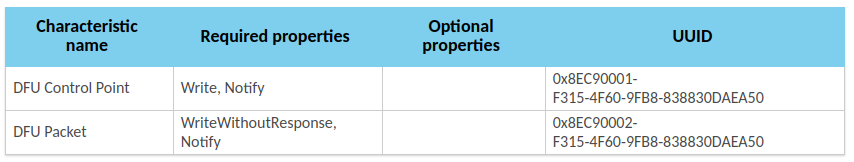
\includegraphics{images/readme/screenshot_20-05-2023_11h25m05.png}
\caption{image}
\end{figure}

Control point procedure operation codes and the respective parameters
and response values:

\begin{figure}
\centering
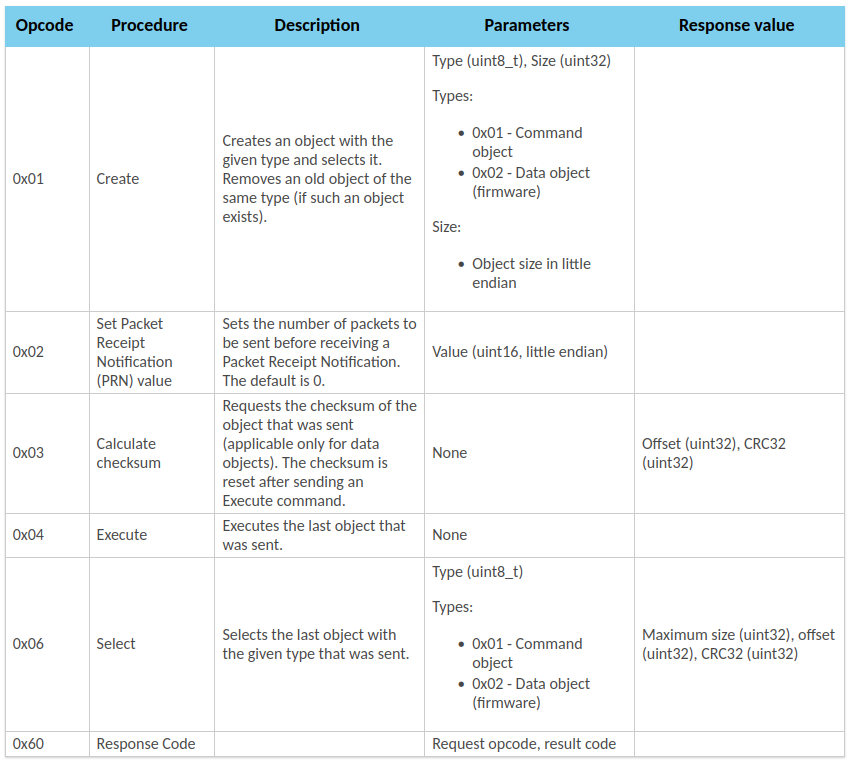
\includegraphics{images/readme/screenshot_20-05-2023_11h26m13.png}
\caption{image}
\end{figure}

The result codes that are sent as part of the response:

\begin{figure}
\centering
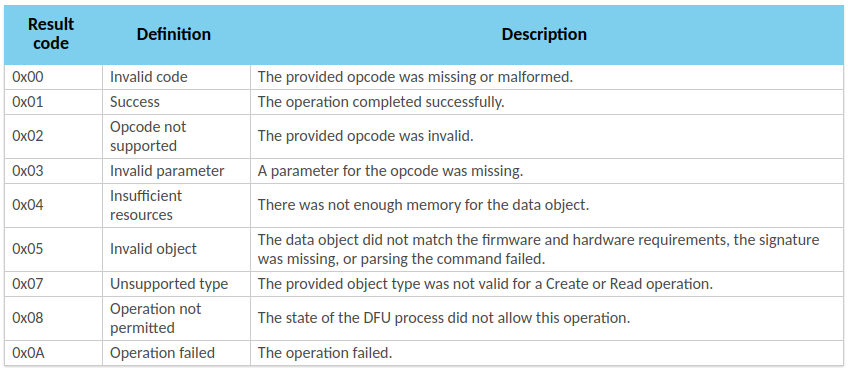
\includegraphics{images/readme/screenshot_20-05-2023_11h36m40.png}
\caption{image}
\end{figure}

\hypertarget{applying}{%
\subsubsection{Applying}\label{applying}}

\begin{itemize}
\tightlist
\item
  0001: trigger the DFU
\item
  0601:

  \begin{itemize}
  \tightlist
  \item
    06: Select
  \item
    01: Create command object
  \end{itemize}
\item
  60 0601 0001 0000 0000 0000 0000 0000:

  \begin{itemize}
  \tightlist
  \item
    60: Response code
  \item
    06: request opcode
  \item
    01: result code
  \item
    0001 0000: Maximum size
  \item
    0000 0000: Offset
  \item
    0000 0000: CRC32, initial value
  \end{itemize}
\item
  02 0000: Set PRN value to be 0
\item
  600201:

  \begin{itemize}
  \tightlist
  \item
    60: Response code
  \item
    02: request opcode
  \item
    01: success
  \end{itemize}
\item
  0101 8d00 0000:

  \begin{itemize}
  \tightlist
  \item
    0101: Create command object
  \item
    8d00 0000: Size in little endian. 0x8d= 141
  \end{itemize}
\item
  600101:

  \begin{itemize}
  \tightlist
  \item
    60: response code
  \item
    01: request code
  \item
    01: success
  \end{itemize}
\end{itemize}

Then the client sends data to the GATT server. Each package maximum size
is 20 bytes which is (MTU-3). There are 7 packages of 20 bytes and one
package of 1 byte. Totaly, there are 141 bytes.

\begin{itemize}
\tightlist
\item
  03: request calculate checksum
\item
  600301 8d000000 c56c4d24:

  \begin{itemize}
  \tightlist
  \item
    60: response code
  \item
    03: request code
  \item
    01: success
  \item
    8d000000: offset
  \item
    c5 6c 4d 24: CRC32
  \end{itemize}
\item
  04: Execute the last object that was sent
\item
  02 0a00:

  \begin{itemize}
  \tightlist
  \item
    02: Set PRN value
  \item
    0a00: little endian, which is 10. It means that client will receive
    a notification every 10 ``write'' commands.
  \end{itemize}
\item
  600201:

  \begin{itemize}
  \tightlist
  \item
    60: response code
  \item
    02: request code
  \item
    01: success
  \end{itemize}
\item
  0602:

  \begin{itemize}
  \tightlist
  \item
    06: select last object
  \item
    02: data object (firmware)
  \end{itemize}
\item
  600601 0010 0000 0000 0000 0000 0000:

  \begin{itemize}
  \tightlist
  \item
    60: response code
  \item
    06: request code
  \item
    01: success
  \item
    0010 0000: maximumsize
  \item
    0000 0000: offset
  \item
    0000 0000: CRC32
  \end{itemize}
\item
  0102 0010 0000:

  \begin{itemize}
  \tightlist
  \item
    01: Create
  \item
    02: Data object
  \item
    0010 0000: Size in little endian: 4096
  \end{itemize}
\item
  600101:

  \begin{itemize}
  \tightlist
  \item
    60: response code
  \item
    01: request code
  \item
    01: success
  \end{itemize}
\end{itemize}

\hypertarget{reverse-app.dat}{%
\subsection{Reverse app.dat}\label{reverse-app.dat}}

\hypertarget{some-examples}{%
\subsubsection{Some examples}\label{some-examples}}

Softdevices 0x1234 - application version 1:

\begin{figure}
\centering
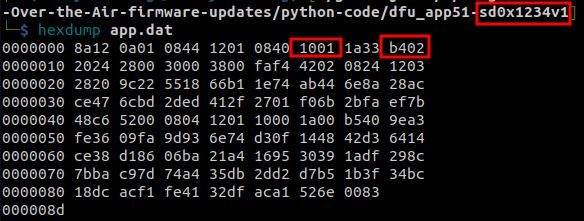
\includegraphics{images/readme/screenshot_21-05-2023_20h36m31.png}
\caption{image}
\end{figure}

Softdevices 0x1111 - application version 1:

\begin{figure}
\centering
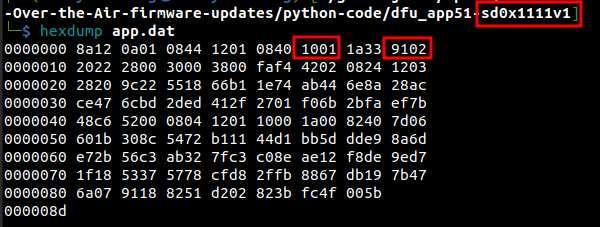
\includegraphics{images/readme/screenshot_21-05-2023_20h37m28.png}
\caption{image}
\end{figure}

Softdevices 0x87 - application version 9:

\begin{figure}
\centering
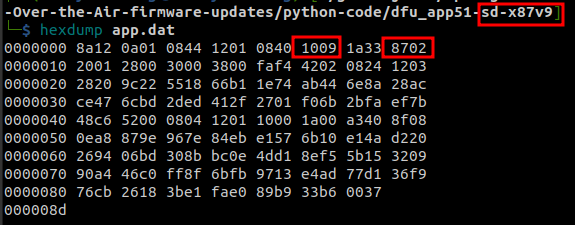
\includegraphics{images/readme/screenshot_21-05-2023_20h38m08.png}
\caption{image}
\end{figure}

Hardware version 52

Softdevices 0x1234 - application version 1:

\begin{figure}
\centering
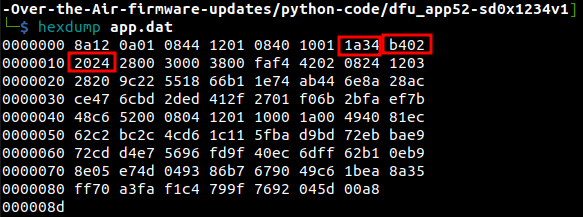
\includegraphics{images/readme/screenshot_21-05-2023_20h45m54.png}
\caption{image}
\end{figure}

\hypertarget{results}{%
\subsubsection{Results}\label{results}}

\begin{figure}
\centering
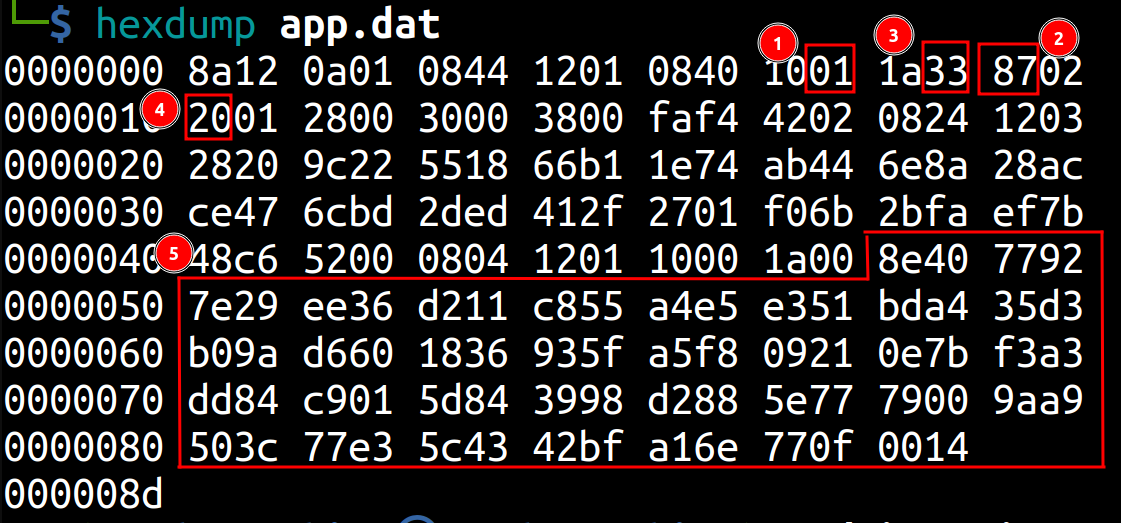
\includegraphics{images/readme/screenshot_21-05-2023_20h52m10.png}
\caption{image}
\end{figure}

\begin{itemize}
\tightlist
\item
  1: application version
\item
  2: softdevice version
\item
  3+4: hardware version
\item
  5: signature of the hash
\end{itemize}

Not sure if these values are two bytes or one byte long.

\hypertarget{how-to-compute-crc32}{%
\subsection{How to compute CRC32:}\label{how-to-compute-crc32}}

nRF5 SDK 12.3.0
\texttt{\textbackslash{}components\textbackslash{}libraries\textbackslash{}crc32\textbackslash{}crc32.c}
